%%%%%%%%%%%%%%%
%
% $Autor: Wings $
% $Datum: 2020-01-29 07:55:27Z $
% $Pfad: TinyMLKit
% $Version: 1785 $
%
%
%%%%%%%%%%%%%%%


\chapter{Tiny Machine Learning Kit}

The Tiny Machine Learning Kit will equip you with all the tools which are needed to start with machine learning. \cite{ArduinoKit:2022}


The kit consists of

\begin{itemize}
    \item an Arduino Nano 33 BLE Sense Lite,  
    \item a camera module OV7675,
    \item USB A to USB Micro B cable, and 
    \item a custom Arduino shield to make it easy to attach components.
\end{itemize}

\begin{figure}[H]
    \centering
    \includegraphics[width=0.9\textwidth]{Nano33BLESense/TinyMLKit/TinyMachineLearningKit.png}
    \caption[Das Tiny Machine Learning Kit]{Das Tiny Machine Learning Kit \cite{ArduinoKit:2022}}
\end{figure}




\section{Das Arduino Tiny Machine Learning Shield}

Das Tiny Machine Learning Shield wird von Arduino für das Tiny Machine Learning Kit hergestellt, um das Verbinden von Komponenten, wie beispielsweise der Kamera, zu vereinfachen. \newline
Bei dem Tiny Machine Learning Shield handelt es sich um ein Breadboard, was speziell für den Arduino Nano 33 BLE Sense ausgelegt ist. Komponenten können entweder wie die Kamera direkt in passende Slots gesteckt oder mit Grove-Kabeln verbunden werden. Außerdem verfügt das Tiny Machine Learning Shield über eine Anschlussklemme, um externe Spannungsquellen anzuschließen und über einen Taster.

\begin{center}

  \begin{tikzpicture}
    \ArduinoNanoShieldTikz
  \end{tikzpicture}    

%    \includegraphics[width=0.9\textwidth]{Nano33BLESense/TinyMLKit/TinyMachineLearningShieldRotated.png}
    \captionof{figure}[Das Tiny Machine Learning Shield]{Das Tiny Machine Learning Shield \cite{ArduinoShield:2021}}
\end{center}

Die Pinbelegung für die Grove-Schnittstellen sind auf dem Tiny Machine Learning Shield beschriftet. Die Belegung für den 10-poligen Steckplatz für die Kamera ist in der Grafik~\ref{TinyMachineLearningShieldPins} dokumentiert.


\begin{center}
    
    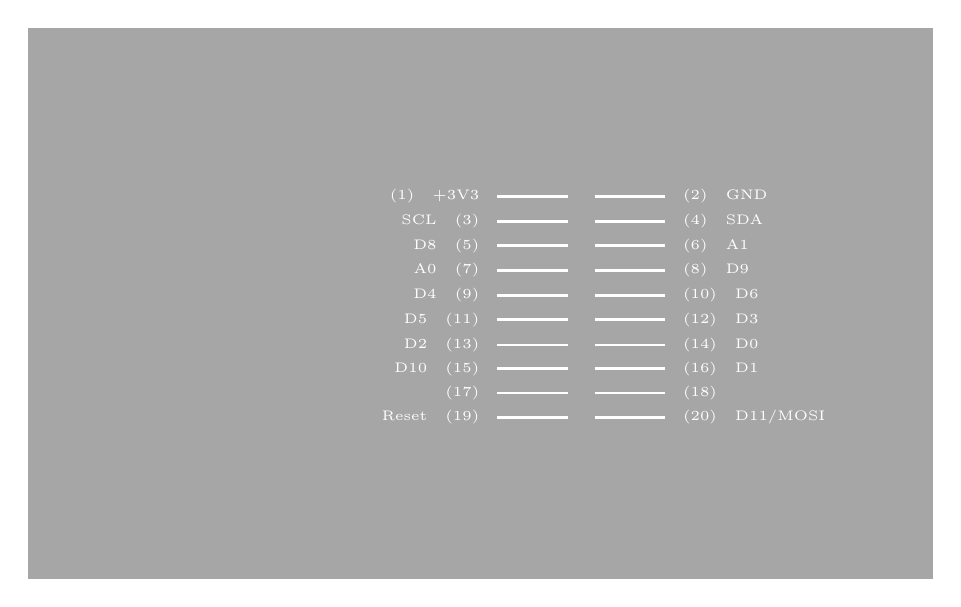
\begin{tikzpicture}
        \ArduinoNanoShieldTikz
        
        \fill[gray, opacity=0.7] (0,30) rectangle (11.5,23);
        
        
        \coordinate (A) at (6.61,28.14);
        \coordinate (B) at (7.45,24.81);    
        \begin{scope}
            \clip (A) rectangle (B);
            
            \ArduinoNanoShieldTikz
            
        \end{scope}
        
        
        %   \fill[black] (6.76, 27.97) rectangle (6.95, 27.76);
        \node[left] (Pin1) at (5.86,27.86) {\textcolor{white}{\tiny (1) \; +3V3}};
        \draw[line width=1pt,white] (6.86,27.86) -- (5.96,27.86);
        
        %   \fill[black] (7.09, 27.96) rectangle (7.29, 27.76);
        \node[right] (Pin1) at (8.2,27.86) {\textcolor{white}{\tiny (2) \; GND}};
        \draw[line width=1pt,white] (7.2,27.86) -- (8.1,27.86);
        
        %   \fill[black] (6.76, 27.64) rectangle (6.95, 27.44);
        \node[left] (Pin1) at (5.86,27.54) {\textcolor{white}{\tiny SCL \; (3)}};
        \draw[line width=1pt,white] (6.86,27.54) -- (5.96,27.54);
        
        %   \fill[black] (7.1, 27.63) rectangle (7.29, 27.44);
        \node[right] (Pin1) at (8.2,27.54) {\textcolor{white}{\tiny (4) \; SDA}};
        \draw[line width=1pt,white] (7.2,27.54) -- (8.1,27.54);
        
        %   \fill[black] (6.77, 27.33) rectangle (6.96, 27.13);
        \node[left] (Pin1) at (5.86,27.23) {\textcolor{white}{\tiny D8 \;  (5)}};
        \draw[line width=1pt,white] (6.86,27.23) -- (5.96,27.23);
        
        %   \fill[black] (7.1, 27.32) rectangle (7.29, 27.13);
        \node[right] (Pin1) at (8.2,27.23) {\textcolor{white}{\tiny (6) \; A1}};
        \draw[line width=1pt,white] (7.2,27.23) -- (8.1,27.23);
        
        %   \fill[black] (6.76, 27.02) rectangle (6.96, 26.82);
        \node[left] (Pin1) at (5.86,26.92) {\textcolor{white}{\tiny A0 \;  (7)}};
        \draw[line width=1pt,white] (6.86,26.92) -- (5.96,26.92);
        
        %   \fill[black] (7.1, 27.01) rectangle (7.29, 26.82);
        \node[right] (Pin1) at (8.2,26.92) {\textcolor{white}{\tiny (8)  \; D9}};
        \draw[line width=1pt,white] (7.2,26.92) -- (8.1,26.92);
        
        %   \fill[black] (6.77, 26.7) rectangle (6.96, 26.5);
        \node[left] (Pin1) at (5.86,26.6) {\textcolor{white}{\tiny D4 \; (9)}};
        \draw[line width=1pt,white] (6.86,26.6) -- (5.96,26.6);
        
        %   \fill[black] (7.1, 26.7) rectangle (7.29, 26.5);
        \node[right] (Pin1) at (8.2,26.6) {\textcolor{white}{\tiny (10) \; D6}};
        \draw[line width=1pt,white] (7.2,26.6) -- (8.1,26.6);
        
        %   \fill[black] (6.77, 26.39) rectangle (6.96, 26.19);
        \node[left] (Pin1) at (5.86,26.29) {\textcolor{white}{\tiny D5 \;  (11)}};
        \draw[line width=1pt,white] (6.86,26.29) -- (5.96,26.29);
        
        %   \fill[black] (7.11, 26.38) rectangle (7.3, 26.19);
        \node[right] (Pin1) at (8.2,26.29) {\textcolor{white}{\tiny (12) \; D3}};
        \draw[line width=1pt,white] (7.2,26.29) -- (8.1,26.29);
        
        %   \fill[black] (6.76, 26.08) rectangle (6.96, 25.87);
        \node[left] (Pin1) at (5.86,25.97) {\textcolor{white}{\tiny D2 \; (13)}};
        \draw[line width=1pt,white] (6.86,25.97) -- (5.96,25.97);
        
        %   \fill[black] (7.1, 26.07) rectangle (7.29, 25.87);
        \node[right] (Pin1) at (8.2,25.97) {\textcolor{white}{\tiny (14) \; D0}};
        \draw[line width=1pt,white] (7.2,25.97) -- (8.1,25.97);
        
        %   \fill[black] (6.76, 25.77) rectangle (6.95, 25.57);
        \node[left] (Pin1) at (5.86,25.67) {\textcolor{white}{\tiny D10 \;  (15)}};
        \draw[line width=1pt,white] (6.86,25.67) -- (5.96,25.67);
        
        %   \fill[black] (7.1, 25.76) rectangle (7.29, 25.57);
        \node[right] (Pin1) at (8.2,25.67) {\textcolor{white}{\tiny (16) \; D1}};
        \draw[line width=1pt,white] (7.2,25.67) -- (8.1,25.67);
        
        %   \fill[black] (6.76, 25.46) rectangle (6.95, 25.26);
        \node[left] (Pin1) at (5.86,25.36) {\textcolor{white}{\tiny (17)}};
        \draw[line width=1pt,white] (6.86,25.36) -- (5.96,25.36);
        
        %   \fill[black] (7.1, 25.45) rectangle (7.29, 25.26);
        \node[right] (Pin1) at (8.2,25.36) {\textcolor{white}{\tiny (18)}};
        \draw[line width=1pt,white] (7.2,25.36) -- (8.1,25.36);
        
        %   \fill[black] (6.76, 25.15) rectangle (6.96, 24.94);
        \node[left] (Pin1) at (5.86,25.05) {\textcolor{white}{\tiny Reset \; (19)}};
        \draw[line width=1pt,white] (6.86,25.05) -- (5.96,25.05);
        
        %   \fill[black] (7.1, 25.14) rectangle (7.29, 24.94);
        \node[right] (Pin1) at (8.2,25.05) {\textcolor{white}{\tiny (20) \; D11/MOSI}};
        \draw[line width=1pt,white] (7.2,25.05) -- (8.1,25.05);
        
        
    \end{tikzpicture}    
    
    %    \includegraphics[width=0.9\textwidth]{Nano33BLESense/TinyMLKit/TinyMachineLearningShieldRotated.png}
    \captionof{figure}[Pin-Belegung des Tiny Machine Learning Shields]{Pin-Belegung des Tiny Machine Learning Shields \cite{ArduinoShield:2021}}\label{TinyMachineLearningShieldPins}
\end{center}





\section{Die OV7675 Kamera}

Da die auf dem Arduino fest verbauten Lichtsensoren nur Helligkeit und Farben messen können, ist in dem Kit eine Kamera enthalten. Diese kann verwendet werden, um Objekte zu erkennen oder einen Videostream auszugeben. In unserem Projekt findet die Kamera allerdings keine Verwendung.\newline
Die Kamera kann direkt auf den mittleren Anschluss des Tiny Machine Learning Shields gesteckt werden. Es sind also keine zusätzlichen Kabel zum Verbinden notwendig. 

\begin{figure}[H]
    \centering
    \includegraphics[width=0.8\textwidth]{Nano33BLESense/TinyMLKit/OV7675.jpg}
    \caption[Das OV7675 Kameramodul]{Das OV7675 Kameramodul \cite{ArduinoKit:2022}}
\end{figure}


\section{USB-Micro-B- auf USB-A-Kabel}

Zur Spannungsversorgung ist in der Box ein USB-Micro-B- auf USB-A-Kabel enthalten. Mit diesem können außerdem die Programme auf den Arduino aufgespielt sowie Daten vom Arduino auf das Programmiergerät übertragen werden.

\begin{figure}[H]
    \centering
    \includegraphics[width=0.8\textwidth]{Nano33BLESense/TinyMLKit/USBCable}
    \caption{Ein USB-A auf Micro-USB Kabel}
\end{figure}
\Mynote{Quelle fehlt}


